\chapter{What is Context?}

While trying to define context for the photo application domain, we found the existing definitions lacking one aspect or another. This is due to their object-centric view of context. In contrast, for an application with scope as broad as photo tagging, this chapter draws emphasis to a relation-centric view of context, and differentiate it from previous object centric definitions. Later, these properties of context are used to specify what objects and relationships are most relevant to the tagging problem.
	
\begin{figure}[h]
\centering
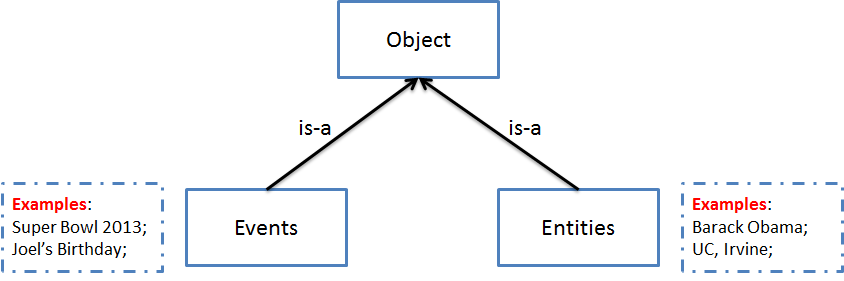
\includegraphics[width=0.6\textwidth]{media/chapter1/terminology.png}
\caption{Objects, Events and Entities.}
\label{fig:terminology}
\end{figure}

Before looking at the different views on context, its advisable to distinguish between `objects' and `entities'. We use the word `Object' to collectively refer to events and entities. The term `object' has been used in literature to refer to things which have no temporal properties. But, in our discussion, an `object' could imply an event which exhibits temporal properties. An entity includes persons, places in the world, for example `Starbucks, UC Irvine', `The Eiffel Tower, Paris, France', or organizations, for example `Google Inc', `Royal Society of London'. Effectively, they are objects which do not need temporal descriptors. Events, on the other hand, are objects which rely on temporal attributes.

\section{Previous Definitons}

One of the earliest studies on context was done by Bill Schilit et al.\ in \cite{schilit1994context}. The focus in this study was how to build software in dynamic environments. The dynamics of the environments were largely due to people requiring different computational services at the different times, the modality of request (through a mobile device or through a workstation), and the environment of the device (are there cameras and projectors nearby if the task requires video conferencing?). This software-centric view of context highlights the importance of two things. One, context is always described with respect to an object. In this case it is the software which runs on processors distributed in a real world environment. Second, context is used to determine how this object interacts with events and entities near it? For example, Schilit uses the example that a workstation should automatically load his favorite text editor when he approaches it; and an rooster music sample must be played whenever fresh coffee is prepared. Both very different and precise interactions even though they might share common background (environment or participating entities). We would not expect a text editor to be shown when coffee is prepared, and the rooster music to be played when an employee walks to a workstation.

\begin{figure}[t]
\centering
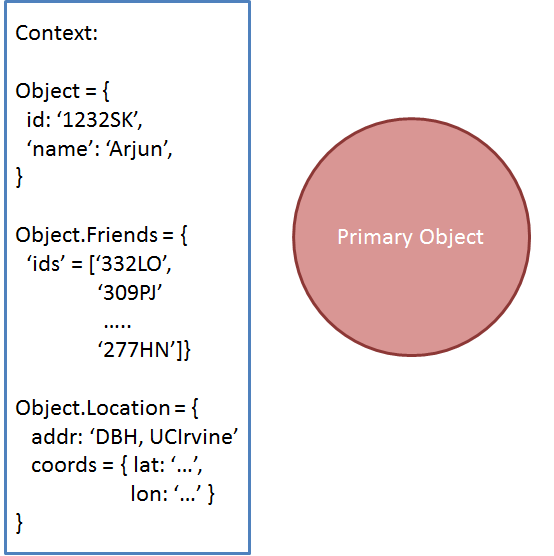
\includegraphics[width=0.5\textwidth]{media/chapter2/dey-def.png}
\caption{Information related to the situation of an Object.}
\label{fig:anind-def}
\end{figure}

In his seminal paper, Anind Dey \cite{dey2001understanding} describes context \textit{as any information that can be used to characterize the situation of an entity. An entity is a person, place or object that is considered relevant to the interaction between a user and an application, including the user and applications themselves}, as shown in figure \ref{fig:anind-def}. He proceeds to explain this definition with the example of an ``indoor mobile tour", arguing that there are there are two additional pieces of information which can be used: \textit{weather} and \textit{presence of other people}. if the user is present with his friends, they might visit sites that are of interest to everybody. There the presence of other people is important context. Because the tour is indoor, weather does not affect the application. It is true that the weather has no direct affect on the application but what about the following scenarios:

\begin{itemize}
\item Could we use the weather information to serve different drinks in the cafeteria to boost the experience of the visitors? On a cold day, placing the hot chocolate kiosk next to the entrance and the ice cream kiosk closer on a warmer day might boost some sales.
\item If the tour is similar to Alcatraz, where a ferry ride takes people to the island, and back from it, a storm brewing in the ocean could lead to disrputed ferry services. Should the application warn its users who are liesurely touring at this time? Or should they continue the tour at the same pace, miss the last ferry and spend the night at Alcatraz? After all, accommodation is not a problem.
\end{itemize}

They then proceed to define Context-Aware computing as follows: \textit{A system is context-aware if it uses context to provide relevant information and/or services to the user, where relevancy depends on the user's tasks}. But, we need to ask ourselves why a system which uses this ``additional information" should be considered a context-aware system? There are numerous systems which would simply consider these ``additional information" as regular inputs. What is different between a system which takes in these inputs as processes them as regular data, and one which processes them as context?

\begin{figure}[t]
\centering
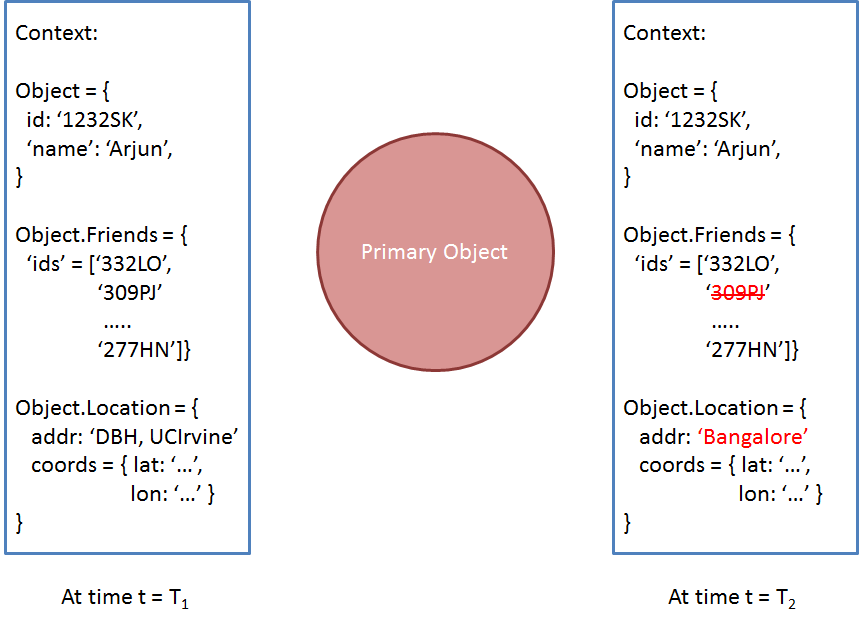
\includegraphics[width=0.75\textwidth]{media/chapter2/ka-obs.png}
\caption{Henricksen's observation about temporality of Context.}
\label{fig:karen-obs}
\end{figure}

Karen Henricksen et al.\ \cite{henricksen2002modeling} make the following interesting observation about context: Context information exhibits a range of temporal characteristics. Some context information can be static, for example the attributes of people using a system (for example, the sex of a person). But a large amount of information is dynamic. For example, the current geo position of a person or her social network, as shown in figure \ref{fig:karen-obs}. There is no straightforward way to obtain this dynamic information other than through sensors. But, such a approach tightly couples the application logic to the types of sensors used, and requires the system to convert the input data to usable representations. For example, the application requires explicit modules to convert GPS coordinates to readable addresses. The problem with such an approach is that there are many ad-hoc modules built to tackle the sensors, and therefore causing the context-awareness to be tied to a specific application.

More recently, Vaninha Vieira et al.\ \cite{vieira2011designing} uses a rule centric view of context to design their context sensitive system, Cemantika. Vaninha defines a contextual element as any piece of data or information which can be used to characterize an entity in an application domain, whereas the context of an interaction between an agent and an application is the set of instantiated contextual elements that are necessary to support the task at hand. Context awareness, for them, is to explicitly switch the task the system is executing under different conditions. For this they explictly model the \textit{context sources} which includes heterogenous and  external sources like sensors, user dialog interfaces and databases. Figure \ref{fig:va-def} shows various data sources providing context. Some data sources are preferred over others depending on certain conditions pre-defined in the system. This allows the various processes to operate independently of the type of sources. It should be noted that the use of ontologies is describing knowledge and context sources is becoming increasingly popular (more similar systems are described in chapter 3).

\begin{figure}[t]
\centering
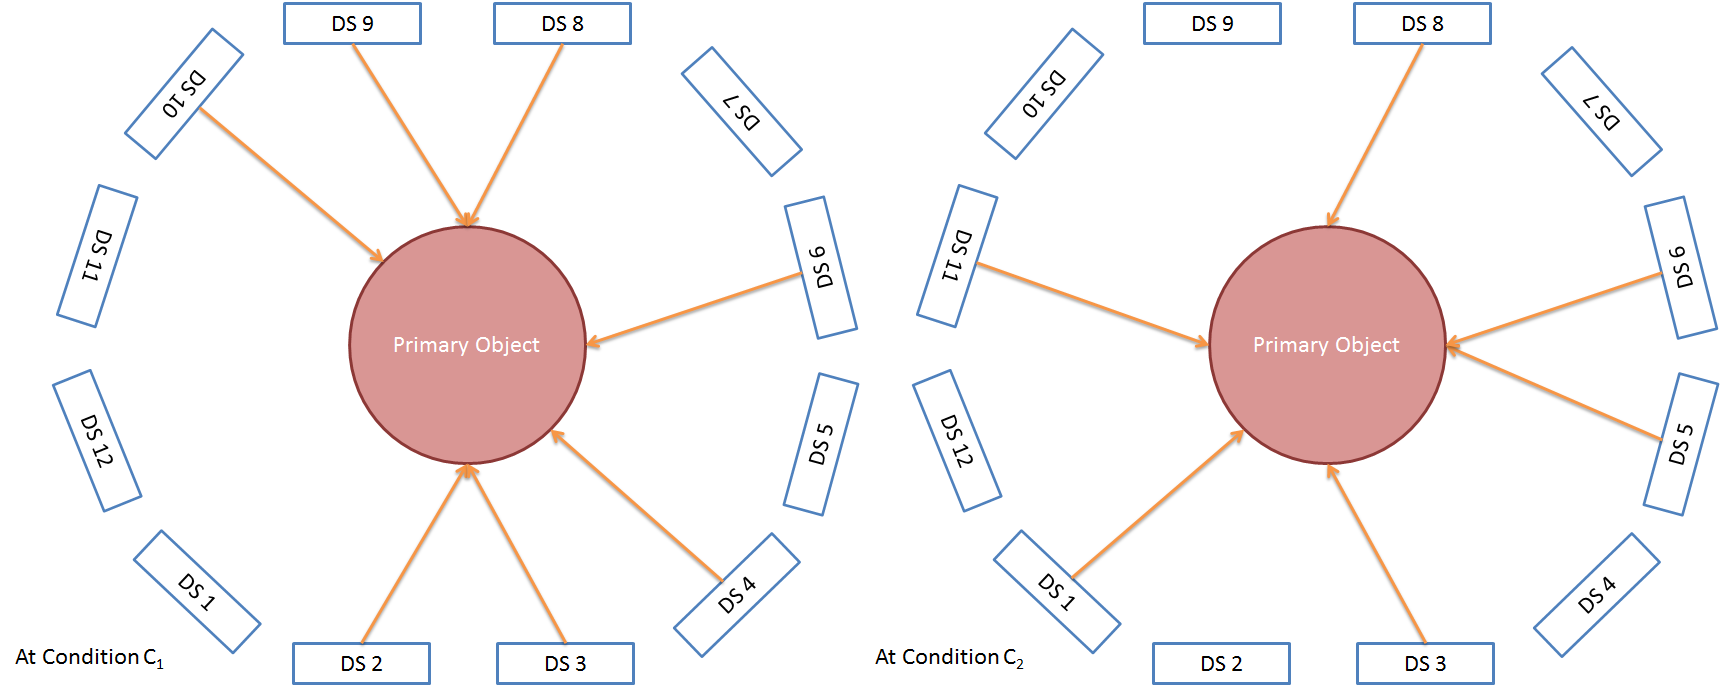
\includegraphics[width=\textwidth]{media/chapter2/va.png}
\caption{Modern context aware system obtain data from different sources.}
\label{fig:va-def}
\end{figure}

\section{Relation-Centric View of Context}

The common ground behind these definitions is their object centric view of context. Context is largely a set of objects that ``surrounds'' a primary object (whose context is in question). This view is insufficient while addressing applications which are very broad in scope, the photo tagging application for example, where users can take photos in very diverse environment, and a large number of sensors and sources of context exist. Specifically, it is non-trivial to identify which subset of available data qualifies to be relevant context for the given photo, and which is not. The two examples from chapter 1, are shown in figures \ref{fig:naaman-icmr} and \ref{fig:example-kasturi-show}. In order to tag the photo on the left, we exclusively used conference calendar information. Whereas, to tag the photo on the right, we used personal information. Our motivation in this chapter is to extend the above definitions of context to allow context aware systems to better extract relevant context from these various sources.

\begin{figure}[t]
\begin{minipage}[b]{0.48\linewidth}
\centering
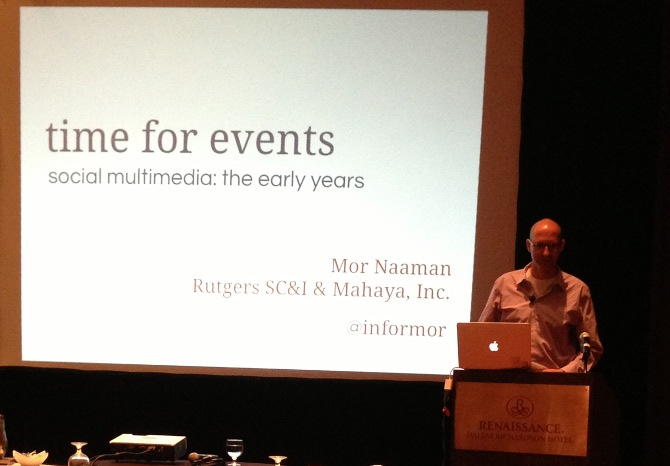
\includegraphics[width=\textwidth]{media/chapter2/naaman.jpg}
\caption{Mor Naaman at ICMR.}
\label{fig:naaman-icmr}
\end{minipage}
\hspace{0.5cm}
\begin{minipage}[b]{0.45\linewidth}
\centering
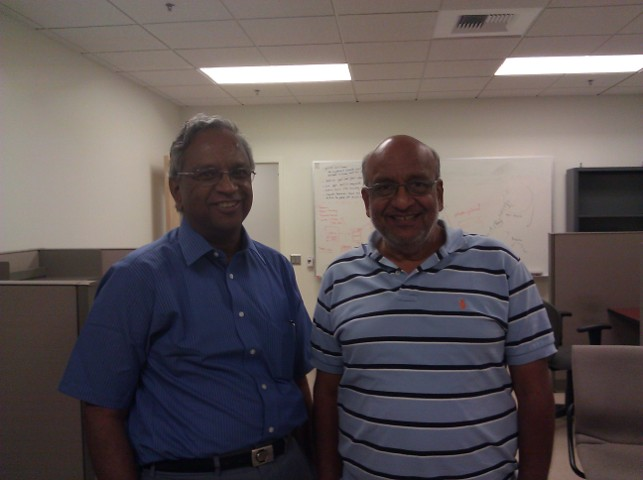
\includegraphics[width=\textwidth]{media/chapter1/kasturi-show.jpg}
\caption{Kasturi and Jain.}
\label{fig:example-kasturi-show}
\end{minipage}
\end{figure}

We define context of a given object at a particular time as \textbf{``the real world information which can be \uline{related to the object directly or indirectly} through a known set of relationships''}. Figure \ref{fig:cn-def} is an extension of \ref{fig:va-def} by making explicit the relations between various objects in the application ecosystem. Here, objects contained within two data sources can be related to each other. For example, an object in DS 9 can be related to another in DS 10 with the \texttt{related-to} edge. The primary object can be related to an object in DS 2 with an \texttt{occurs-at} relationship at time $t_1$. Whereas at time $t_2$, the relationship with DS 2 does not exist, but a new relationship \texttt{occurs-during} surfaces with DS 11.

\begin{figure}[t]
\centering
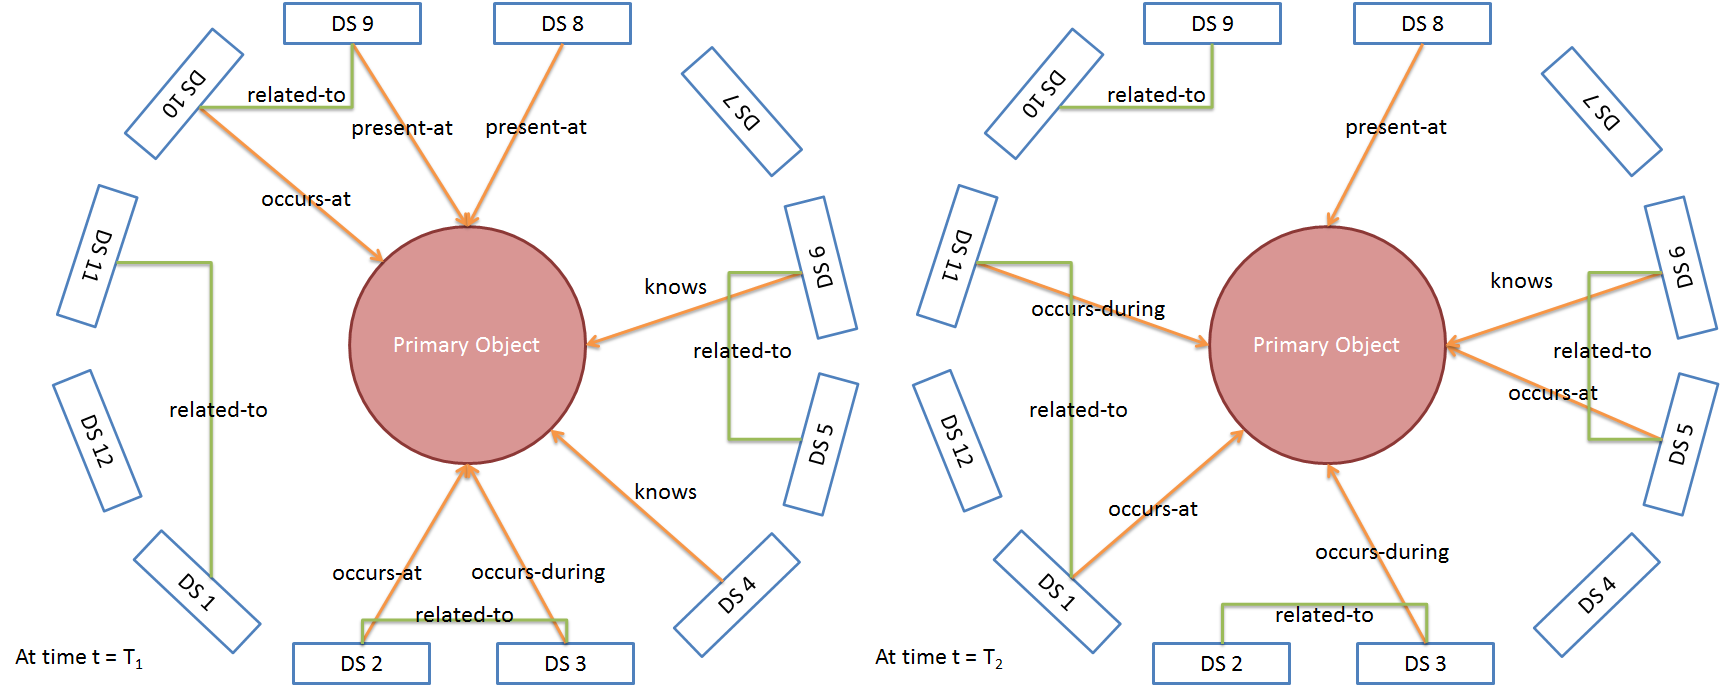
\includegraphics[width=\textwidth]{media/chapter2/cn.png}
\caption{Utilizing relations to define context for the primary object.}
\label{fig:cn-def}
\end{figure}

Relationships can be of different types. They can be simple labels like \texttt{friend-of} signifying a social relationship. Or they can more actionable like \texttt{located-at}, which relates a person to a particular location, and therefore causes a particular audio stream to play through the handheld device. This relation is not just a label, it imposes constraints on the properties of objects which it relates. Here, the spatial attributes of the the person and the exhibit must match if they are being related through a \texttt{located-at} attribute. In this dissertation, we will see that such relations, which impose such property constraints are critical in algorithmically determining which information is relevant context. Let us also assume that we have available to us the four types of data sources: event sources, place databases (like yelp.com), weather information sources and social networking information.

Using this relation centric view, we now look at how the examples from chapter 1 can be formulated in a systematic process to discover context. A system to discover context must establish a set of relationships its context objects can be connected with. For the two photos, we choose \textbf{participant-of}, which indicates that an entity is a participant in an event, and \textbf{subevent-of} which indicates that an event is occurring within another super-event. Thus, any entity can be related to other events through a \texttt{participant-of} edge, and events can be related to others events as well as entities through \texttt{subevent-of} and the \texttt{participant-of} edge respectively.

\begin{figure}[ht!]
\begin{minipage}[b]{0.48\linewidth}
\centering
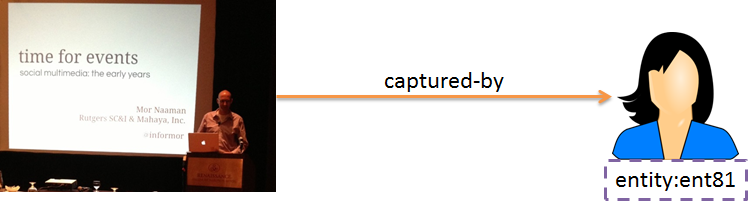
\includegraphics[width=\textwidth]{media/chapter2/naaman-1.png}
\caption{Primary objects.}
\label{fig:naaman-example-1}
\end{minipage}
\hspace{0.5cm}
\begin{minipage}[b]{0.45\linewidth}
\centering
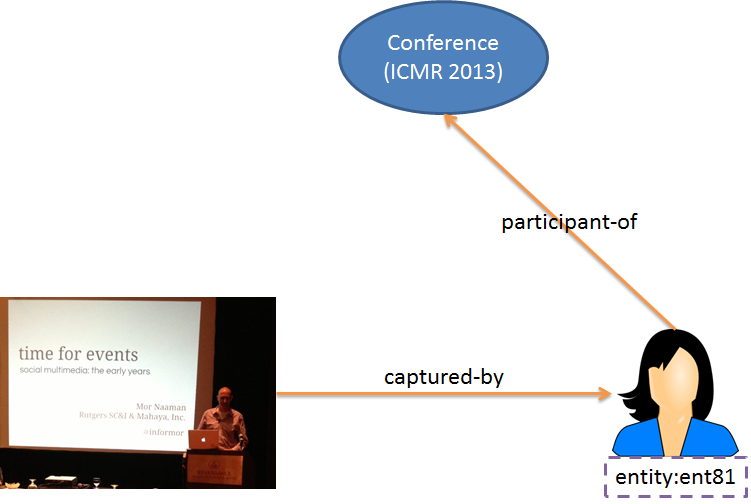
\includegraphics[width=\textwidth]{media/chapter2/naaman-2.png}
\caption{Associating \texttt{conference event} using the \texttt{participant-of} relation}
\label{fig:naaman-example-2}
\end{minipage}
\begin{minipage}[b]{0.48\linewidth}
\centering

\includegraphics[width=\textwidth]{media/chapter2/white.png}
\label{fig:naaman-example-x}
\end{minipage}
\hspace{0.5cm}
\begin{minipage}[b]{0.45\linewidth}
\centering

\includegraphics[width=\textwidth]{media/chapter2/white.png}
\label{fig:naaman-example-y}
\end{minipage}
\begin{minipage}[b]{0.48\linewidth}
\centering
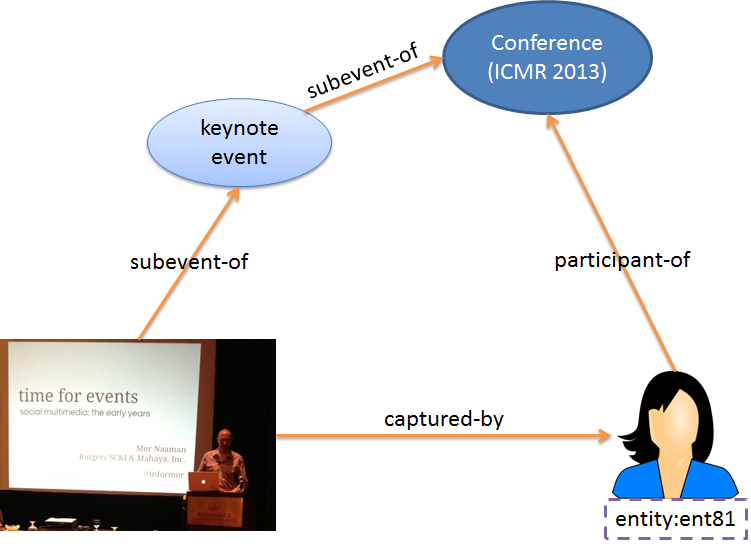
\includegraphics[width=\textwidth]{media/chapter2/naaman-3.png}
\caption{Associating the keynote event.}
\label{fig:naaman-example-3}
\end{minipage}
\hspace{0.5cm}
\begin{minipage}[b]{0.45\linewidth}
\centering
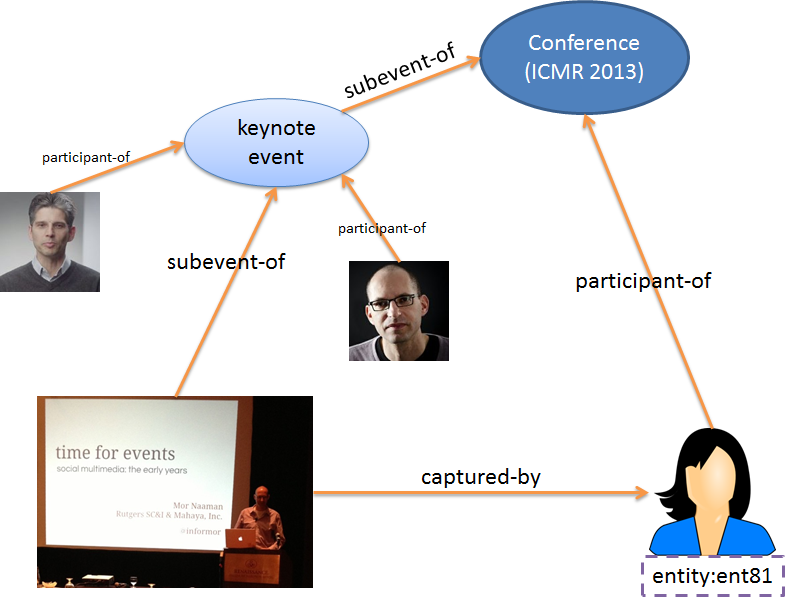
\includegraphics[width=\textwidth]{media/chapter2/naaman-4.png}
\caption{Associating the participants using the \texttt{participant-of} relation}
\label{fig:naaman-example-4}
\end{minipage}
\end{figure}

Figures \ref{fig:naaman-example-1} through \ref{fig:naaman-example-4} show how the two relationships can be used to gather context for the photo in figure \ref{fig:naaman-icmr}. Figure \ref{fig:naaman-example-1} shows the initial graph created using the \texttt{photo-capture-event} and the photographer, \texttt{entity:ent81}. Figure \ref{fig:naaman-example-2} shows the result of adding context by associating an event with \texttt{entity:ent81}. Given this new graph with three nodes, a context aware system can find more context by trying to find objects which can be related through the two edges. Since one of the nodes is a \texttt{conference} event, it proceeds to find events occurring within it, and adds the keynote event, which also happens to be the super-event of the \texttt{photo-capture-event}. The result is shown in figure \ref{fig:naaman-example-3}. Finally, the keynote event is extended with relations to associate subevents or participants. In this case, the only new context available are the participants of the keynote event. These two entities are associated with the event as shown in figure \ref{fig:naaman-example-4}. 

In the above example, given a graph containing primary objects, we grew it by relating objects from the real-world using a fixed set of relationships \{\texttt{participant-of}, \texttt{subevent-of}\}. Such a graph representing the primary objects, the context objects and their inter-relationships is a \textbf{context network}. Figure \ref{fig:context-network} shows one such context network for Mor Naaman's photo taken at ICMR 2013. A similar procedure can be invoked on the photo in figure \ref{fig:example-kasturi-show} to discover its context network.

Because of the type of relationships chosen, some information which was readily available (weather, place or social networking, for example) was not associated. But if we extend the relationship set to contain another relation \texttt{occurs-at}, then the place where the conference was held will be included in the context network. Similarly, the inclusion of a \texttt{knows} can relate entities with each other. If the social networking source reports that \texttt{entity:ent81} was a friend of Mor Naaman, an additional edge would be introduced between these nodes in the context network. Thus, relations are key in determining which objects are context and which are not, and how they are related to the primary objects.

\begin{figure}[h]
\centering
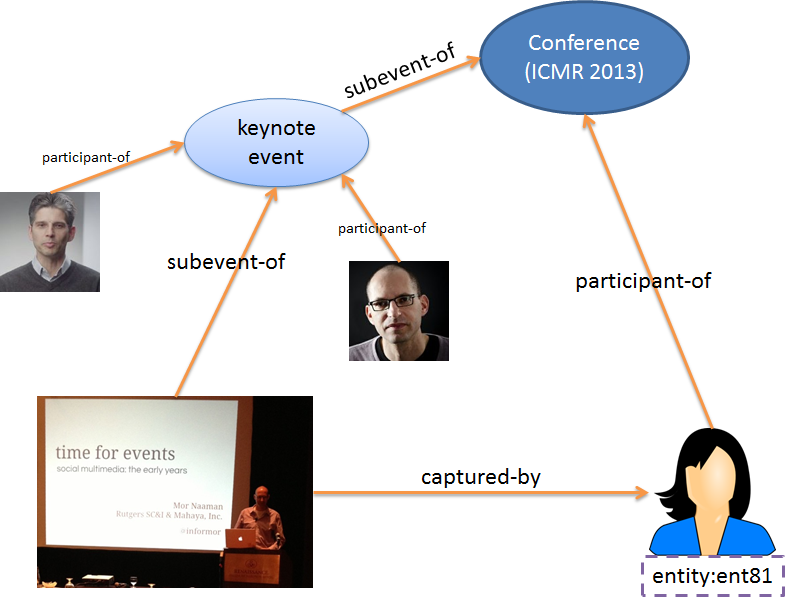
\includegraphics[width=0.75\textwidth]{media/chapter2/naaman-4.png}
\caption{Context Network for Mor Naaman's photo.}
\label{fig:context-network}
\end{figure}

\section{Modeling Context}

It must be noted that asserting the need for a relation-centric view of context is not discounting the importance of objects. Rather, it is a way of saying that relationships are atleast as important as objects are. Keeping this in mind, we will see what are the primitives required to model context for real-world problems in this section.

\subsection{Object Types and Semantics}

Context is always specified with respect to a real world object. This primary object must be uniquely identifiable in the computational system, and must be an instance of one of the known classes. This object must have some real world attributes. For example, if the object is an event, then the interval during which it occurs, and location of occurence are two real world attributes. In the tour guide application, the visitor is one possible primary object whose context needs to determined. In the photo application, possible types of interest include the \texttt{photo-capture-event}, the \texttt{photographer}, various possible events which can occur in the world, people and places where photography can occur.

Different objects bring with them very specific semantics. While modeling objects as context, these semantics must be preserved. For example, an event object exists only for a fixed time interval. Entities can only be present at one place at one point in time. In the later chapter, we will see that these axiomatic properties play a very important role in the context discovery algorithm.

\subsection{Relationships and Constraints}
Context is any event or entity which can be \textit{related} to the objects in a problem. Instead of finding objects which are of a specific type, and qualifying them as context, objects related to the problem variables through specific relationship types are to be considered context. These relationships can impose certain constraints on the objects which they relate. For example, the subevent relation requires that the super-event spatio-temporally contain the smaller event. Such constraints are very common in real-world relationships. Many examples can be seen in applications involving chemical reactions, where it is not sufficient to have just two reactants at the same time and place, but the reaction could demand very specific environmental factors (like temperature or pressure). The specification of the relationships for modeling context should permit the specification of these specific constraints.

\subsection{Temporal Semantics}
Among the various constraints a relationship can impose, many of them are temporal. The subevent relationship asserts a very specific constraint between the temporal attributes of the two events it relates. Modeling context requires the ability to express relationships which assert such temporal constraints. Temporal relations have been studied in literature, and can be reused for the purpose \cite{allen1983maintaining, wolter2000spatio}.

\subsection{Spatial Semantics}
Similarly, spatial constraints between objects in a context network need to modeled. For example, the subevent relationship asserts the constraint that the super-event must spatially contain the sub-event.

\section{Properties of Context-aware System}

Context-awareness of a system is its \textbf{``ability to explore different types of information to identify context relevant to the objects in its ecosystem, and using this context to reduce the complexity of a given task''}. 

\subsection{Real-World Knowledge}
Modeling real world knowledge (what are the different objects in the world, and how do they precisely interact with each other) is critical in context based systems. This is in contrast with rule based systems, where a set of real world conditions are sensed to trigger a particular action. Examples of knowledge are: An academic conference has atleast one keynote talk; or Sodium reacts with atmospheric oxygen at room temperature; or water expands when it freezes. A network of knowledge constitutes the model for a context based system. This paves the way of it to expand its knowledge about the current situation of the primary object based on what is already known about the object, and what is needed. For example, if an Object is associated with a keynote talk, data about the co-occuring conference should be obtained. Alternatively, if the system had associated a conference with the object, data about the keynote must be sought out. This `guiding light' trait of knowledge is a pre-requisite in a context-aware system.

\subsection{Dynamic Linking}
The relation centric view, and temporal relevance properties lead us to how the primary object is linked to different sources in the environment. If the primary object is linked to all sources in the environment, we say that it \textit{statically links} to these sources. For example, if the tour guide application which brings in data from all sources all times. On the other hand, dynamic linking with only relevant sources has the ability to restrict input from many sources, and therefore be more capable in future ecosystems where thousands of sensors from the web or in the local network are availble. Also, such a design allows system developers to add more sources in the case of ``Black Swan'' events, which were not foreseen before, but are now posing a challenge to the performance of the system.

Also, context has been used in many non-real world problems. For instance, in natural language processing \cite{lee1990context}, ranking pages of the web \cite{page1999pagerank}, entity resolution \cite{chen2009exploiting}, face clustering in images \cite{zhang2013unified} and therefore it must not mean that contextual techniques must apply only to real world problems. For the purposes of this dissertation, we ignore the application of context in such problems.



%%% Combine this section with the previous one?

% \section{Modeling Primitives}

% \subsection{Types}

% \subsection{Models}

% \subsection{Relationships and Constraints}






% \section{Parallels}
% The real world is very big. Modeling it can be a very hard task. Do we really need such large and elaborate models if we are to call our application ``context-aware"? In this section, we look at how \textit{contextual thinking}\cite{capra1997web} has helped understand, and in some cases solve, many of the long standing problems in different disciplines. We will start with an anecdotal example, and move to more elaborate examples which demonstrate how to reason in real world problems. The reason for this section is to justify the need for modeling many different types of real world information, which is a pre-requisite for employing context based techniques. 

% \subsection{Black Swans}
% In his widely acclaimed book, The Black Swan\cite{taleb2010black}, Nassim Nicholas Taleb presents many arguments against solely relying on prediction based techniques. Citing examples from stock markets to clinical psychology trials he presents the case that historical evidence is insufficient to position oneself in the future. 

% His example of a turkey brings to light an interesting point ``Consider a turkey that is fed every day. Every single feeding will firm up the bird's belief that it is the general rule of life to be fed every day by friendly members of the human race \textit{looking out for its best interest}. On the afternoon of the Wednesday before Thanksgiving, something unexpected will happen to the turkey. It will incur a revision of belief.''

% Any amount of prediction is futile in this case. Taleb plots the graph \ref{fig:turkey} showing the belief of the turkey in mankind. How could the turkey protect itself, yet reaping the benefits of the food given to it? 

% The answer lies not in developing complex techniques about reasoning what is already known. But to look at the problem from different vantage points. From the standpoint of the turkey, the Wednesday event is a Black Swan event. But from the standpoint of the butcher, it is not, since its occurrence is not unexpected. So, if the turkey explores the world around it, it will soon reach a point where it is able to reason the nature of human behavior, their customs, and finally arrive at the conclusion, that there exists one such custom which is absolutely disastrous for the turkey's well being.

% The simple example shows how new objects bring with them different semantics. And highlights that interactions can be disrupted heavily with even the slight change in relations. The second thing it shows is the need for awareness in the turkey to ``look-out'' for potential causes of harm. This action of being context-awareness is criticial in any real world systems.

% \begin{figure}[t]
% \centering
% 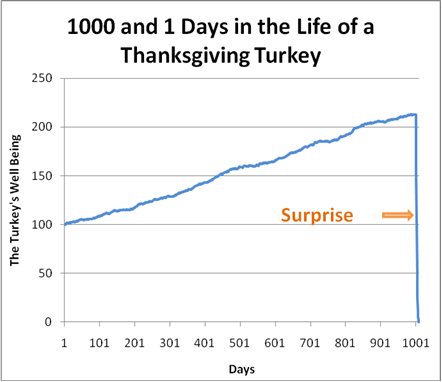
\includegraphics[width=0.75\textwidth]{media/chapter2/turkey.png}
% \caption{Expectations of a Turkey as Thanksgiving approaches.}
% \label{fig:turkey}
% \end{figure}

% \subsection{Context in History}
% Historians love context. Almost all their works heavily rely on finding interesting events in a particular timeframe which can explain the events that followed. In his book, Guns, Germs and Steel \cite{diamond1997guns}, Jared Diamond argues the need to understand specific environmental diversities, and use them to reason why history happened the way it did. We are familiar with the conquest story of the Inca emperor Atahuallpa by the Spanish conquistador Francisco Pizzaro at Cajamarca, Peru in 1532\cite{wiki:spanishconquest}. Historians attribute the success of Pizzaro to better Spanish ammunition and warfare techniques. But the more interesting question is \textit{Why was Pizzaro at Cajamarca conquering the Incas, and not Atahuallpa crossing the Atlantic to conquer Spain?} Effectively, how did South Americans evolve so different from Europeans? The answer, it turns out, lies in different environmental conditions.

% Diamond outlines the various steps that led to such cultural diversity in a flowchart similar to \ref{fig:axis-flowchart}. Let us see how he arrived at it. Any conflict usually favors the party with a stronger political, military, economic and social structure. The South American society consisted of the high ranking chiefs who were treated as Gods, and were the only people permitted to read and write. Everyone else was engaged in the daily activities of food production. Thus, a majority of the man power was spent in solving the daily food problem. There was no scope for any organizations to develop which would construct and develop military and economic disciplines. On the other hand, these organizations not only existed in Europe, but also \textit{co-existed} each other, thereby driving each other to be more mature and stronger. The stronger organizations led to creation of stronger ammunition (guns, steel, sword), transport services (ships which could travel across the atlantic), writing technology (since everyone in Pizzaro's army was capable of communicating messages through time and space).

% \begin{figure}[t]
% \centering
% 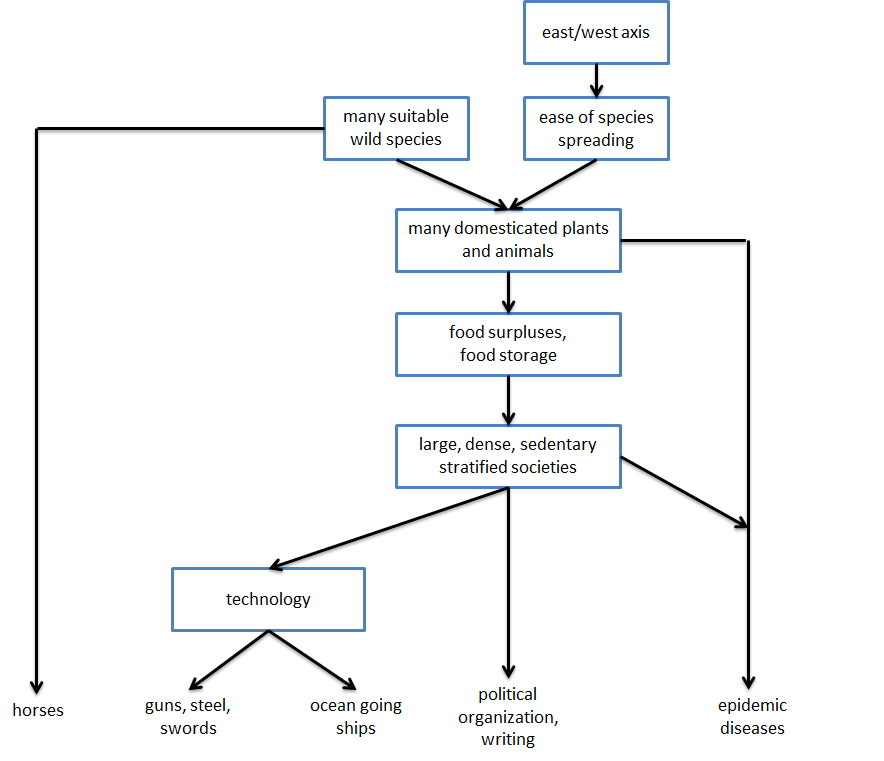
\includegraphics[width=\textwidth]{media/chapter2/axis.png}
% \caption{Reasons for diversity among cultures.}
% \label{fig:axis-flowchart}
% \end{figure}

% \textbf{Why did the Europeans form such a stratified society, and not the South Americans?} The majority of the south americans were concerned about procuring food for the next day. Food production systems in Europe reached a critical peak, because of which they developed technology for storing food. Because day-to-day food was no longer a concern, a significant section of the population now was ``free'' to indulge in other activities. This led to development of art, policital, military units, economic systems, which in turn evolved each.

% \textbf{Why did food production reach an all time high in Europe and not in South America?} The reason lies in three environmental factors: the soil, flora and fauna of the area and how they interacted over a larger time span. Europe and Asia has been home to a more diverse set of animals and plans. Since 6000B.C., farmers and animals of the area were able to choose from this bigger variety of plants, and evolve them over thousands of years to form better crops. The role of a larger set of animals in the area is interesting too. Over the years, Europeans have domesticated most of the animals than people from any part of the world. Big mammals like cows and bulls were found in plenty in Europe and Asia. This led to much higher yields than tilling the soil by hand. Regions like South America lacked such variety of domesticable animals. For example, there is no point in domesticating an elephant, as it takes 14-15 years to reach adulthood and be of use. Animals like Rhinos are very strong, and therefore, can be excellent farm animals, but are very hard to tame (in fact they are extremely dangerous). These reasons led the South Americans to rely only on man power to tackle the daily food problem.

% \textbf{Finally, why did biodiversity emerge in Europe/Asia, and not in the Americas or Africa?} Thousands of years ago, the biggest deterrent in sustaining life was the climate. People lived nomadic lifestyles which came in contact with different weather, and acclimatizing to it required almost a reboot of their knowledge, environmental know-how and customs. Now, lets take a look at the map of the world, shown in \ref{fig:continental-axis} -- what do we see? Europe and Asia span longitudinally, whereas Americas and Africa extend along the Earth's latitude. What is the biggest advantage this offers Eurasians? When they moved from place to place, the structure of their continent allowed them to move to places with \textbf{similar weather}. This allowed them to move to different regions and enjoy the same weather, grow similar crops and domesticate the same animals. But people in Africa or America had to move out of their comfort zone, and move to area containing different weather and biodiversity, and had to redo everything from scratch. Effectively, cultures which could move freely without rebooting their knowledge found it easier to develop than others.

% \begin{figure}[t]
% \centering
% 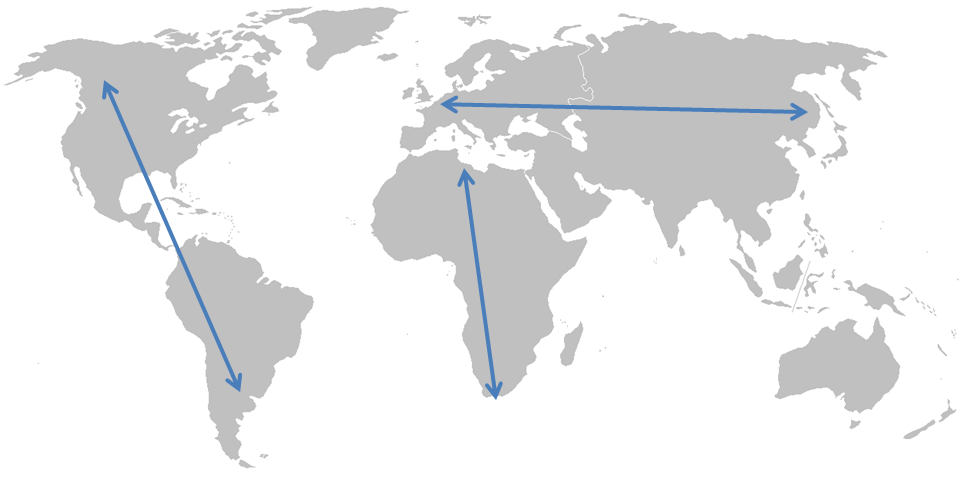
\includegraphics[width=\textwidth]{media/chapter2/continents-e.png}
% \caption{Horizontal/vertical extents of different continents.}
% \label{fig:continental-axis}
% \end{figure}

% There is also this idea that cultures which had to undergo such reboots frequently had to deal with more complexities of the world, and could rely less on objective knowledge, and therefore made people rely more on religious principles to lead their lives. This led to prevalence, and eventually domination by religious organizations.

% % http://pocketcultures.com/topicsoftheworld/files/2009/06/map-importance-of-religion-by-country.png

% % http://en.wikipedia.org/wiki/File:Religion_in_the_world.PNG

% Diamond's book is an exploration of the broadest pattern of history. What it tells us is that explicit modeling of real world objects with their native properties are extremely important in reasoning about the world.

% \subsection{The Gaia Hypothesis}
% Charles Darwin's work describes how living being have evolved over billions on years. But it does not answer the question -- how does life sustain itself on Earth? It turns out that the few billion years of life we have had is too little to let life have evolved randomly, and just let natural selection determine who succeeds. There had to be other factors which let life sustain and grow in specific ways.

% One of the theories put forward by James Lovelock and Lynn Margulis in the 1970s, more commonly known as the Gaia Theory, proposes the presence of natural feedback loops to explain the sustanence of life\cite{margulis1974biological}. Their argument is that for life to sustain, the amount of carbon dioxide in the atmosphere must not exceed a certain threshold. But who keeps this in check? How has the amount of $CO_2$ in the atmosphere been almost constant for the last millions of years. Their reasoning is as follows:

% The Earth's volcanoes have spewed out huge amounts of carbon dioxide for millions of years. Plant and animals recycle massive amounts of $CO_2$ in the process of photosynthesis, respiration and decay. According to the Gaia theory, the excess of $CO_2$ is recycled by a vast feedback loop, which involves rock weathering as a key ingredient. Rainwater washes atmospheric $CO_2$ onto rocks. In the process of rock weathering, rocks, rainwater and $CO_2$ form chemicals known as carbonates. The carbonates are then washed down where tiny algae invisble to the naked eye, absorb them and use them to make shells of chalk. So the $CO_2$ that was in the atmosphere has now ended up in the shells of those minute algae. In addition, ocean algae also absorb $CO_2$ from the surface of the ocean.

% When the algae die their shells are then washed down into the ocean, where they form sediments of limestone. Limestone is very heavy, and gradually sinks into the mantle of the earth. Eventually, some of the $CO_2$ is released back to the atomsphere by volcanoes. The entire cycle -- linking volcanoes to rock weathering, to soil bacteria, to oceanic algae, to limestone sediments, and back to volcanoes -- acts as a feedback loop which regulates the Earth's temperature. It turns out that bacteria in the soil vastly increases the rate of rock weathering (acting as a catalyst). In the sun gets hotter, the bacteria in the soil get higher than average ambient temperature, which causes them to increase the rock weathering activity, causing more $CO_2$ to be removed from the atmosphere and sent to the ocean, thus cooling the planet.

% This remarkable explanation involves rocks, bacteria and ocean dynamics and the even the sun to explain how earth's temperature is regulated. By studying one or more objects in isolation makes the analysis far from complete. More interestingly, the relations between the objects are very precise, involving specific biochemical reactions within some acceptable ambient conditions.

% \subsection{Significance}
% These examples are not to present here to report the latest advances in different disciplines, but to glance at how reasoning is done in the real world. Both the use cases require very precise knowledge of relations between different objects in the world (for example, how the sun can affect bacterial growth in the soil), and have access to a large amount of sensors and data sources. Once these two have been established, the computational challenge is how to form accurate models of the models of the world, and how to use those models to either reduce the complexity of the problem so a human can operate with ease, or apply additional algorithms to solve the problem. 

% In the next section, we see what we types of information we shall consider as context for the problem of tagging personal photos.

\section{Context for Personal Photos}
Our justification for the use of context begins with the statement: \textit{For a given user, the correctness of face tags for a photograph containing people she has never met is undefined}. This observation prepares us to understand what context is, and how contextual reasoning assists in tagging photos. The description of any problem domain requires a set of abstract data types, and a model of how these types are related to each other. We \textbf{define} contextual types as those which are semantically different from these data types, but can be directly or indirectly related to them via an extended model which encapsulates the original one. Contextual reasoning assists in the following two ways. \textbf{First}, contextual data restricts the number of people who might appear in the photographs. We can also argue that all the personal data of a user (her profile on Facebook, LinkedIn, email exchanges, phone call logs) provides a reasonable estimate of all these people who might appear in her photos. \textbf{Second}, by reasoning on abstractions in the contextual domain, we can infer conclusions on the original problem. We exploit this property to develop our algorithm in the later sections. Though CueNet can be applied to a variety of recognition problems, we focus on tagging people in personal photos for concreteness, where, the image and person tag form the abstractions in the problem domain. The types used in the contextual domain, but not limited to, are the following:

\begin{itemize}
\item \textbf{Event Objects}: includes description of events like conferences, parties, trips or weddings, and their structure (for example, what kind of sessions, talks and keynotes are occurring within a particular conference).
\item \textbf{Entity Objects}: information about a user's social graph, people whom she corresponds with using email and other messaging services.
\item \textbf{Geographical Objects}: various tools like Facebook Places, Google Latitude or Foursquare provide information about where people are at a given time.
\end{itemize}

The important relations which dealing with such data are:

\begin{itemize}
\item \textbf{Subevent Relation}: If two events occur such that, one spatio-temporally contains the other, we say that it is the subevent of the one with larger spatio-temporal span. For example, a talk event is a subevent of the conference during which it happens.
\item \textbf{Participation Relation}: If an entity is participating in an event, s/he is said to be a participant-of that event. Note that this relation constraints the spatio-temporal boundary where the entity could be present during the interval of the event.
\item \textbf{Social Relation (knows)}: Social relations relate people who are acquainted with each other. This is used to model social networking information obtained from sources like Facebook or Email.
\item \textbf{Spatio-Temporal Relations}: Events occur in specific time intervals, and at some location. We use the relations occurs-at and occurs-during to model these properties. More details are provided in the next chapter.
\end{itemize}

The above classes of contextual data can be obtained from a variety of data sources. Examples of data sources range from mobile phone call logs and email conversations to Facebook messages to a listing of public events at upcoming.com. We classify sources into the following types:

\begin{itemize}
\item \textbf{Personal Data Sources}: include all sources which provide details about the particular user whose photo is to be tagged. Some common examples of personal data sources include Google Calendar, Email and Facebook profile and social graph.
\item \textbf{Social Data Sources}: include all sources which provide contextual information about a user's friends and colleagues. For example, LinkedIn, Facebook and DBLP are some of the commonly used websites with different types of social graphs.
\item \textbf{Public Data Sources}: include all sources which provide information about public organizations (like restaurants, points of interest or football stadiums) or about public events (like fairs, concerts or sports games).
\end{itemize}

Social and public data sources are enormous in size, containing information about billions of events and entities. Trying to use them directly will lead to scalability problems faced by face recognition and verification techniques. But, by using personal data, we can discover which parts of social and public sources are more relevant. For example, if a photo was taken at San Francisco, CA (where the user lives), his family in China is less relevant. Thus, the role of personal information is twofold. \textbf{Firstly}, it provides contextual information regarding the photo. \textbf{Secondly}, it acts as a bridge to connect to social and public data sources to discover interesting people connected to the user who might be present in the event and therefore, the photo.

At this point we should revisit the \textbf{temporal relevance} property of a data source. Given a stream of photos taken during a time interval, the source which contributed interesting context for a photo might not be equally useful for the one appearing next. This is because sources tend to focus on a specific set of event types or relationship types, and the two photos might be captured in different events or contains persons with whom the user maintains relations through different sources. For example, two photos taken at a conference might contain a user's friends in the first, but with advisers of these friends in the next. The friends might interact with the user through a social network, but their advisers might not. By using a source like DBLP, the relations between the adviser and friends can be discovered. We say that the temporal relevance of these context sources is \textbf{\textit{low}}. This requirement will play an important role in the design of our framework, as now, sources are not hardwired to photo, but instead need to be discovered gradually.

In chapter 4, we will see how these different objects, relations and data sources are used by out context-aware framework to assist tagging faces in personal photos.